%%%%%%%%%% Aquí va el código.
\subsection*{Pregunta 4.}
Considera el siguiente autómata
\begin{multicols}{2}
\begin{center}
  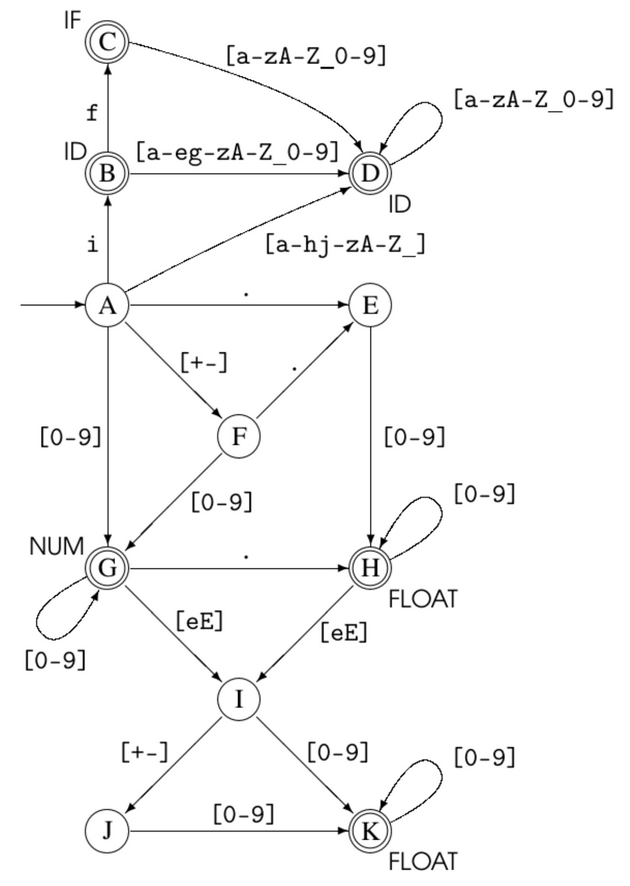
\includegraphics[scale=0.30]{./Automata.png}
\end{center}

\begin{itemize}
\item[$a$)] ¿Cuál es la definición del lenguaje que acepta este autómata?
  Proporciona la gramática regular de los tokens que se reconocen.
\item[$b$)] ¿Qué tokens son reconocidos al procesar la cadena 3e-z? Recuerda
  utilizar la técnica de la coincidencia más larga y si no es posible avanzar
  en un estado puedes hacer un retroceso o backtracking al estado de aceptación
  anterior para tratar de identificar el mayor número de tokens posible.
\end{itemize}
\end{multicols}

\textbf{Solución.} 
\begin{itemize}
\item[$a$)] 
\item[$b$)] Para este inciso usemos el método visto en clase, así
  \begin{enumerate}
  \item Encontramos la cadena ``3e-'' del token pasando por los estados [A $\rightarrowtriangle$
    G $\rightarrowtriangle$ I $\rightarrowtriangle$ J], al llegar a J realizamos backtracking para
    llegar a I, pues no encontramos una transición que nos permita encontrar z desde j. Caso análogo
    para I, G, y finalmente llegamos a el estado A.
  \item Encontramos ``e'' por la transición A $\rightarrowtriangle$ D. Sin embargo, no podemos encontrar
    el siguiente caracter del token y hacemos backtracking llegando nuevamente al estado inicial (A).
  \item Encontramos ``-'' por la transición A $\rightarrowtriangle$ F. Sin embargo, no podemos encontrar
    el siguiente caracter del token y hacemos backtracking llegando nuevamente al estado inicial (A).
  \item Encontramos ``z'' por la transición A $\rightarrowtriangle$ D. Sin embargo, no podemos encontrar
    el siguiente caracter del token y hacemos backtracking llegando nuevamente al estado inicial (A).
  \end{enumerate}
\end{itemize}
%\[/* \left([\text{\textasciicircum} *\: /] | \left([\text{\textasciicircum} *] /\right)^{\star} |
% \left([\text{\textasciicircum} /] *\right)^{\star} | [\text{\textasciicircum} * /]^{+}\right)^{\star} [*]^{\star}*/\]
